\section{The design}
\label{design}

We propose to solve the image sentiment analysis with the convolutional neural network to detecting mid-level representations. We use an AlexNet-styled network and perform a two-stage training scheme where the network first learns the noun part of mid-level representations. Then we rearrange the dataset and train the network with triplet loss to force the network to learn the adjective part. 

\subsection{Preliminary}
We adopt the Adjective Noun Pairs (ANP) proposed in \cite{borth2013large} as the mid-level representations for image sentiment analysis. ANPs are frequently found in practice and reflect strong sentiment. Each ANP contains exactly one adjective and noun word, such as "beautiful flower" or "creepy house". 

We use polarized sentiment model that each image can either be classified as positive or negative. 

\subsection{Network structure}

\begin{figure}[h]
    \centering
    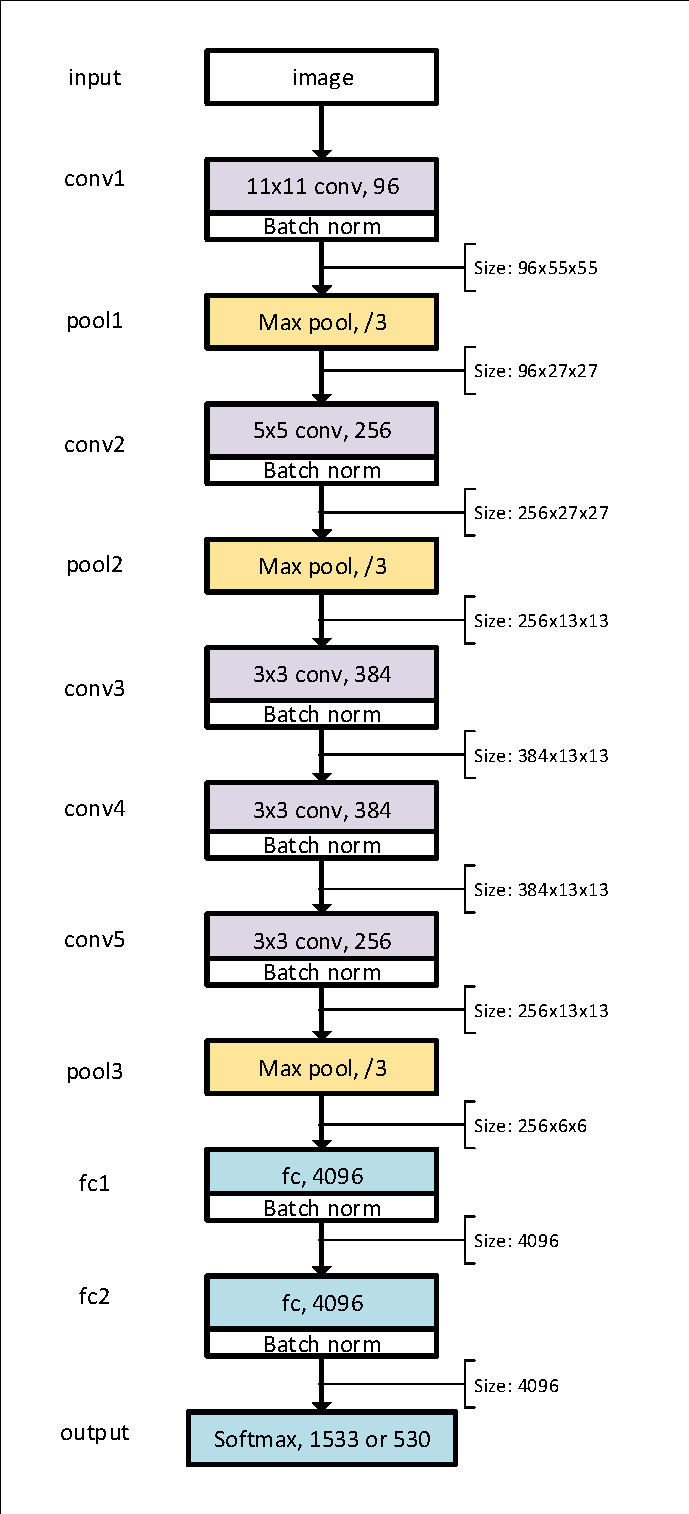
\includegraphics[width=\linewidth]{./figures/network.pdf}
    \caption{Network structure}
    \label{fig:net_structure}
\end{figure}

Here we show the architecture of our convolutional neural networks. The network contains 5 convolutional layers and 2 fully connected layers with a softmax layer as the output layer. There are max-pooling layers at the first, second and last convolutional layers. Batch normalization is performed before activation for each convolutional layers and fully connected layers. ReLU is used as the activation function for all layers. Adam \cite{kingma2014adam} is used as the optimizer of the network. We use cross entropy and triplet loss as the loss function for each training stage respectively. The detailed size of each layer is shown in Figure \cite{fig:net_structure}

\subsection{Two stage training}
It is widely shown in the literature \cite{krizhevsky2012imagenet, szegedy2015going, simonyan2014very, he2016deep} that convolutional neural networks are good at image classification tasks. In \cite{campos2017pixels}, the authors have shown that convolutional neural networks pre-trained on image classification datasets can be quite effective at image sentiment prediction tasks. So in our work, we adopted a two-stage training scheme that let the network learn the noun and adjective part of ANPs gradually.

The first stage of training is let the network learn the noun part of ANPs. This stage is the same as the image classification task. We first extract all noun words from all ANPs. Then we set the last softmax layer with the size of the number of noun words and use cross-entropy loss to train the network.

The second stage requires us to modify the network structure and the loss function. We first replace the softmax layer with a new one that has the size of the number of ANPs and initialize it randomly. Then we replace the loss function with triplet loss and train the network again using images from the same dataset.
To train triplet, the data need to be arranged in triplets, each triplet consist of an anchor point, a positive point from the same class of the anchor point, and a negative class from a different class than anchor point. The triplet loss is defined below, where $D$ is the distance between different data points and $m$ is the margin to ensure the network does not form trivial models where distances of all pairs of data points are $0$.

\[
\mathcal{L}_{tri}(\theta) = \sum_{a,p,n} [m + D_{a,p} - D_{a,n}]_{+}.
\]

To training with triplet loss, a crucial step is to mining good triplets as there are $n^3$ number of possible triplets when the dataset contains $n$ data points. If the selected triplets are too simple, the network will stop learning quickly. However, if the triplets are too hard, the network will become unstable \cite{hermans2017defense}. To ensure the network learn meaningful information from the training, we arrange the dataset in a way that in each triplet, all three image belongs to the same noun class. However, the negative image has the different ground truth ANP with the anchor image and the positive image. For example, we may select both the anchor image and positive image from "beautiful flower", and select a negative image from "dead flower". Ideally, the negative image should have the different sentiment as the anchor point. There are cases where a noun class only has one ANP or has all ANPs with the same sentiment, but even though we can hardly select meaningful triplets to train the network in such a case, the network will not suffer from it when predicting sentiment of the image.

When the network finished training, it can classify images to ANPs. Then with the ANP, we can predict the sentiment of the image. A simple solution would be predicting the sentiment of the image with the ANP with the highest probability of the softmax output layer. However, in many cases, it is more robust to use top-k ANPs with the highest probability of softmax layer. For example, it is very common that there are multiple ANPs in a single image, sometimes even with a different sentiment, or the top ANP prediction is not correct. 